\newpage
\section{Implémentation de différents modèles}

Après avoir réalisé la classification par champs lexical et s’être rendu compte que cette méthode ne fonctionné pas nous nous sommes orientés vers plusieurs classification.











\subsection{SVM (Support Vector Machine)}

Pourquoi SVM ? Avec plusieurs tests, SVM semble être le plus précis (voir section \ref{comparaison}).  
Les différents paramètres établis pour ce modèle sont test\_size=0.1 et train\_size=0.5 (voir section \ref{variation_SVM})

\begin{center}
    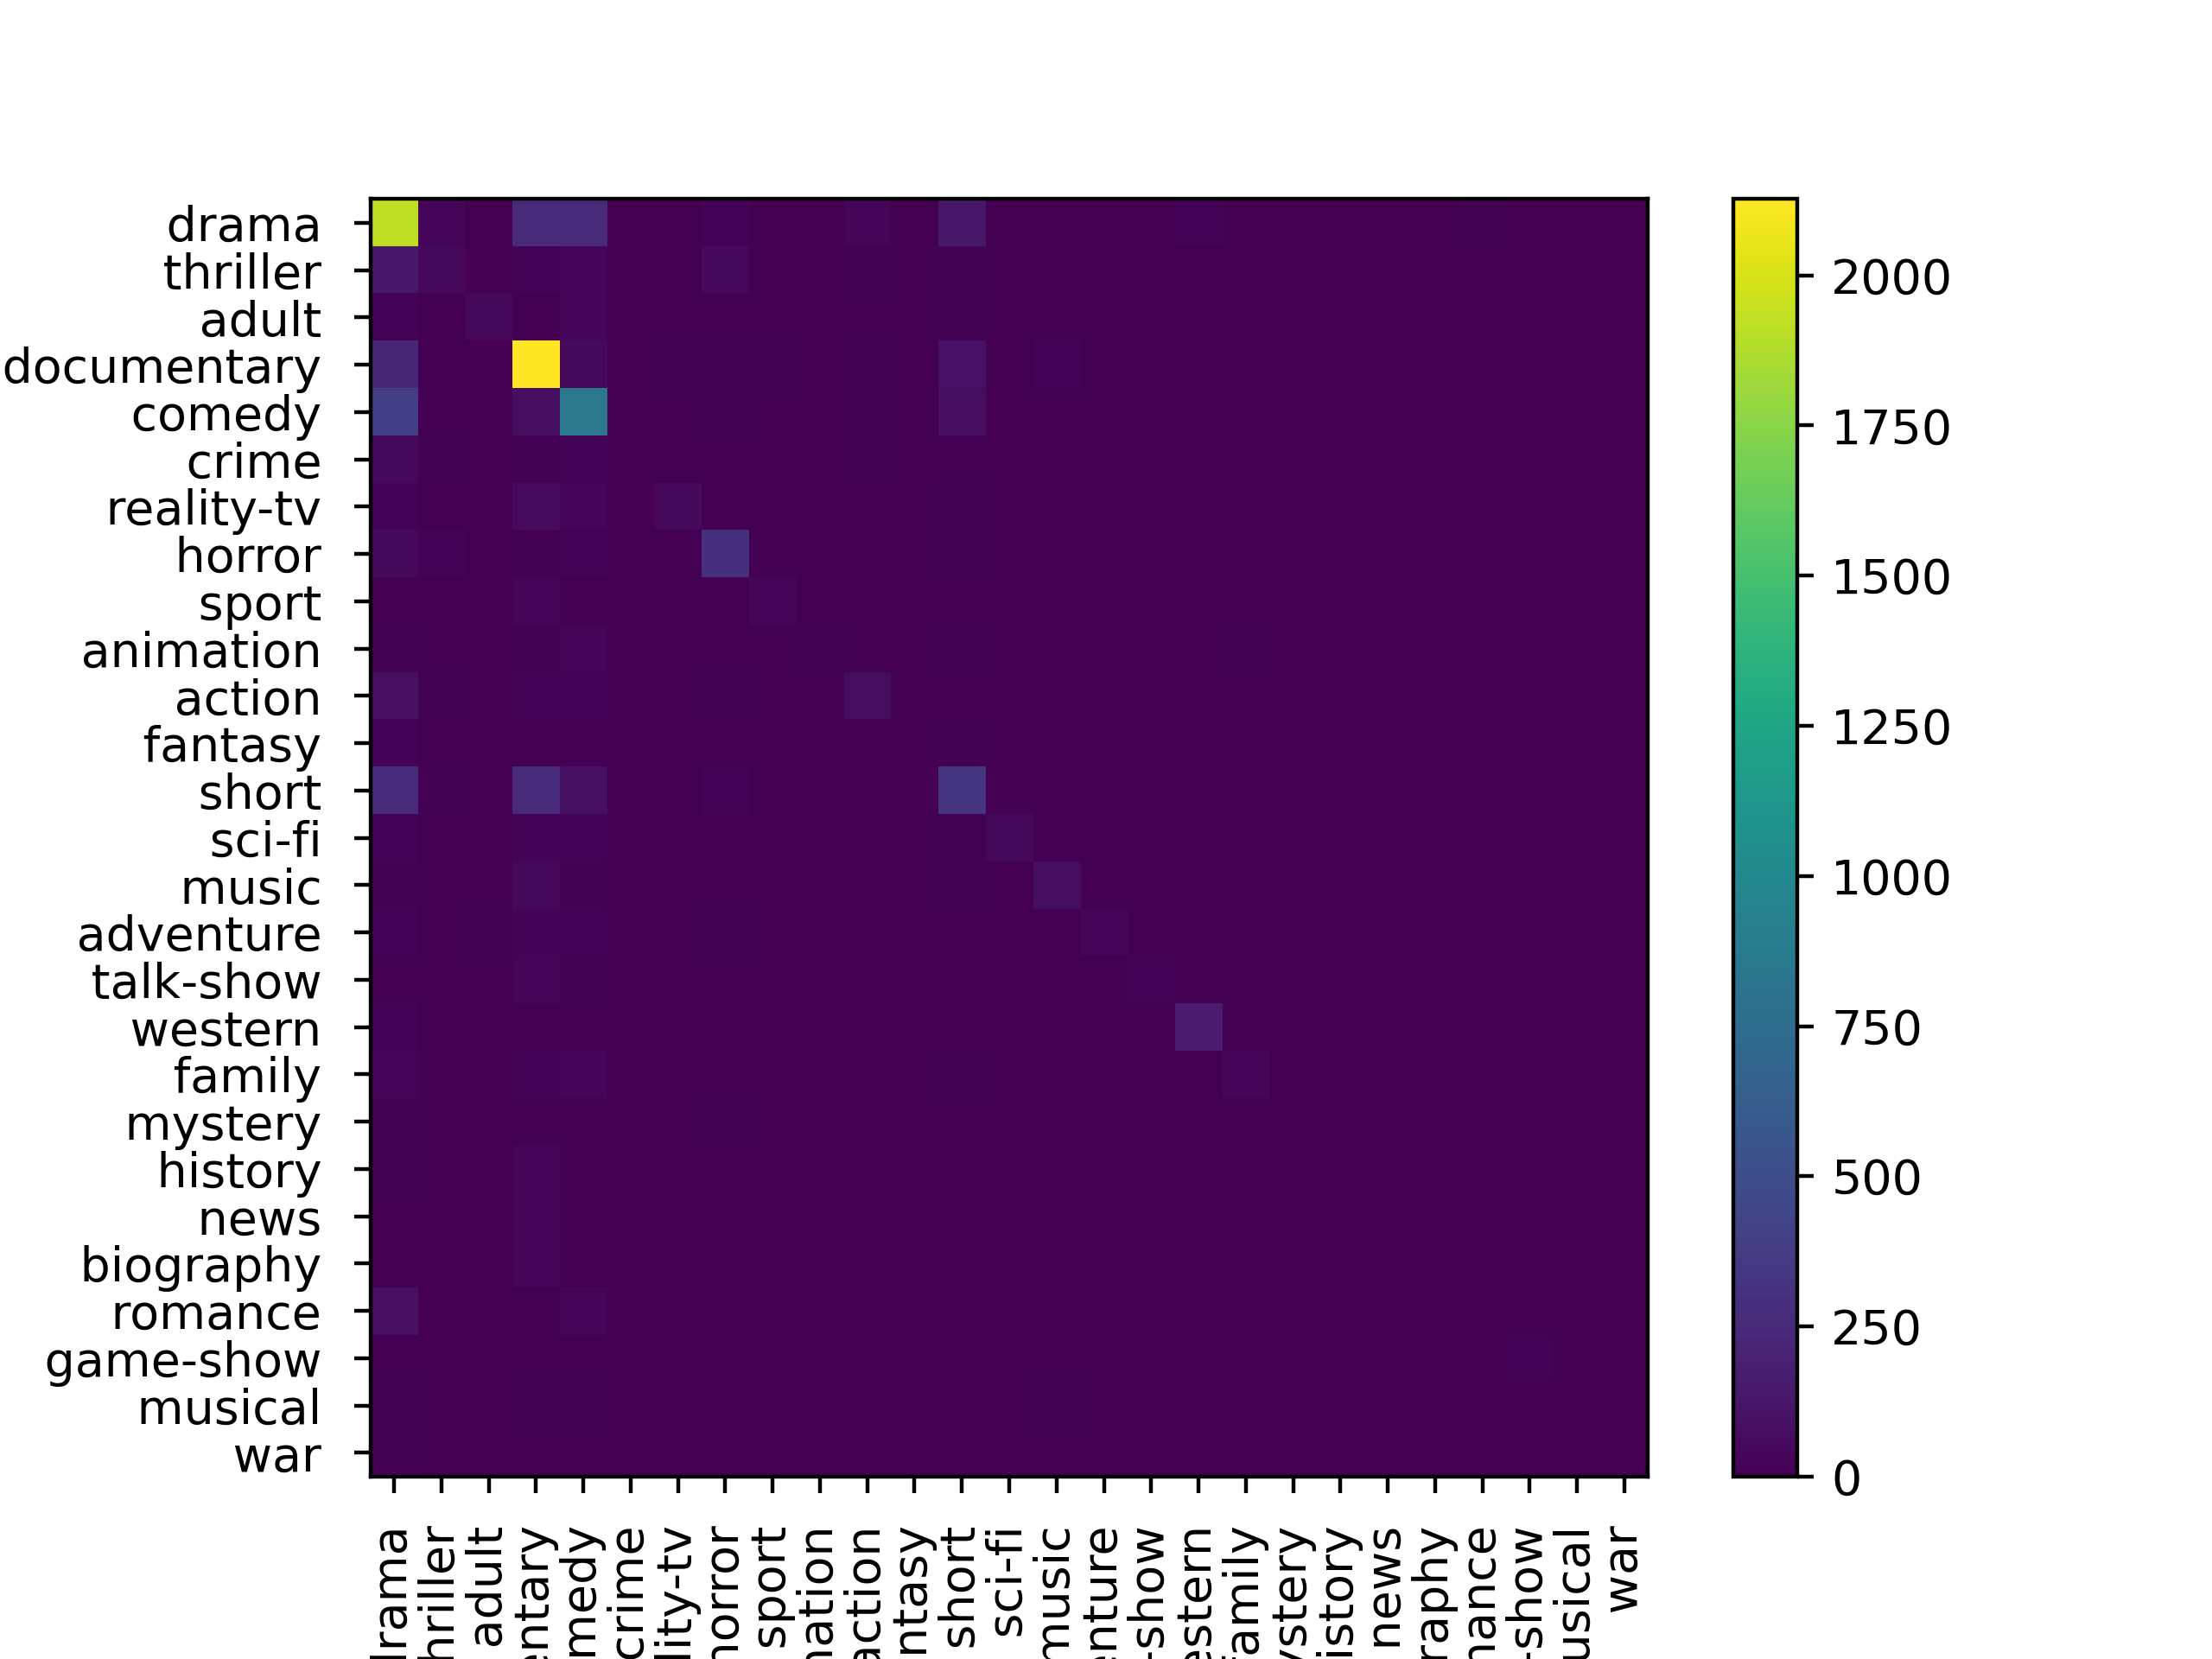
\includegraphics[scale=1]{graphs/confusion_matrix_LinearSVC().png}
    \captionof{figure}{Matrice de Confusion SVM}
\end{center}

Dans la matrice de confusion ci-dessus, il y a \textbf{Drama} et \textbf{Documentary} qui nous pose problème, ces 2 genres sont énormément confondu avec d'autres.













\newpage
\subsection{LogisticRegression}

D'après notre comparaison SVM semblais être le meilleur modèle malgré cela il est très long à entrainer. Comme à ce moment-là nous n'avions pas encore trouvé comment enregistré un model (ce référé section \ref{model}) nous voulions essayer une autre méthode. C’est pourquoi nous avons implémenté LogisticRegression.\\
La LogisticRegression est un algorithme de classification. Il est utilisé pour prédire un résultat binaire basé sur un ensemble de variables indépendantes.\\



Pour ce modèle nous avons attribué respectivement aux variables test\_size et train\_size les valeurs 0.2 et 0.7 (ce référé section \ref{variation_LogisticRegression}). Avec ces paramètres nous avons une accuracy de 58\% ainsi qu'un taux d'erreur légèrement supérieur à 42\%.

\begin{center}
    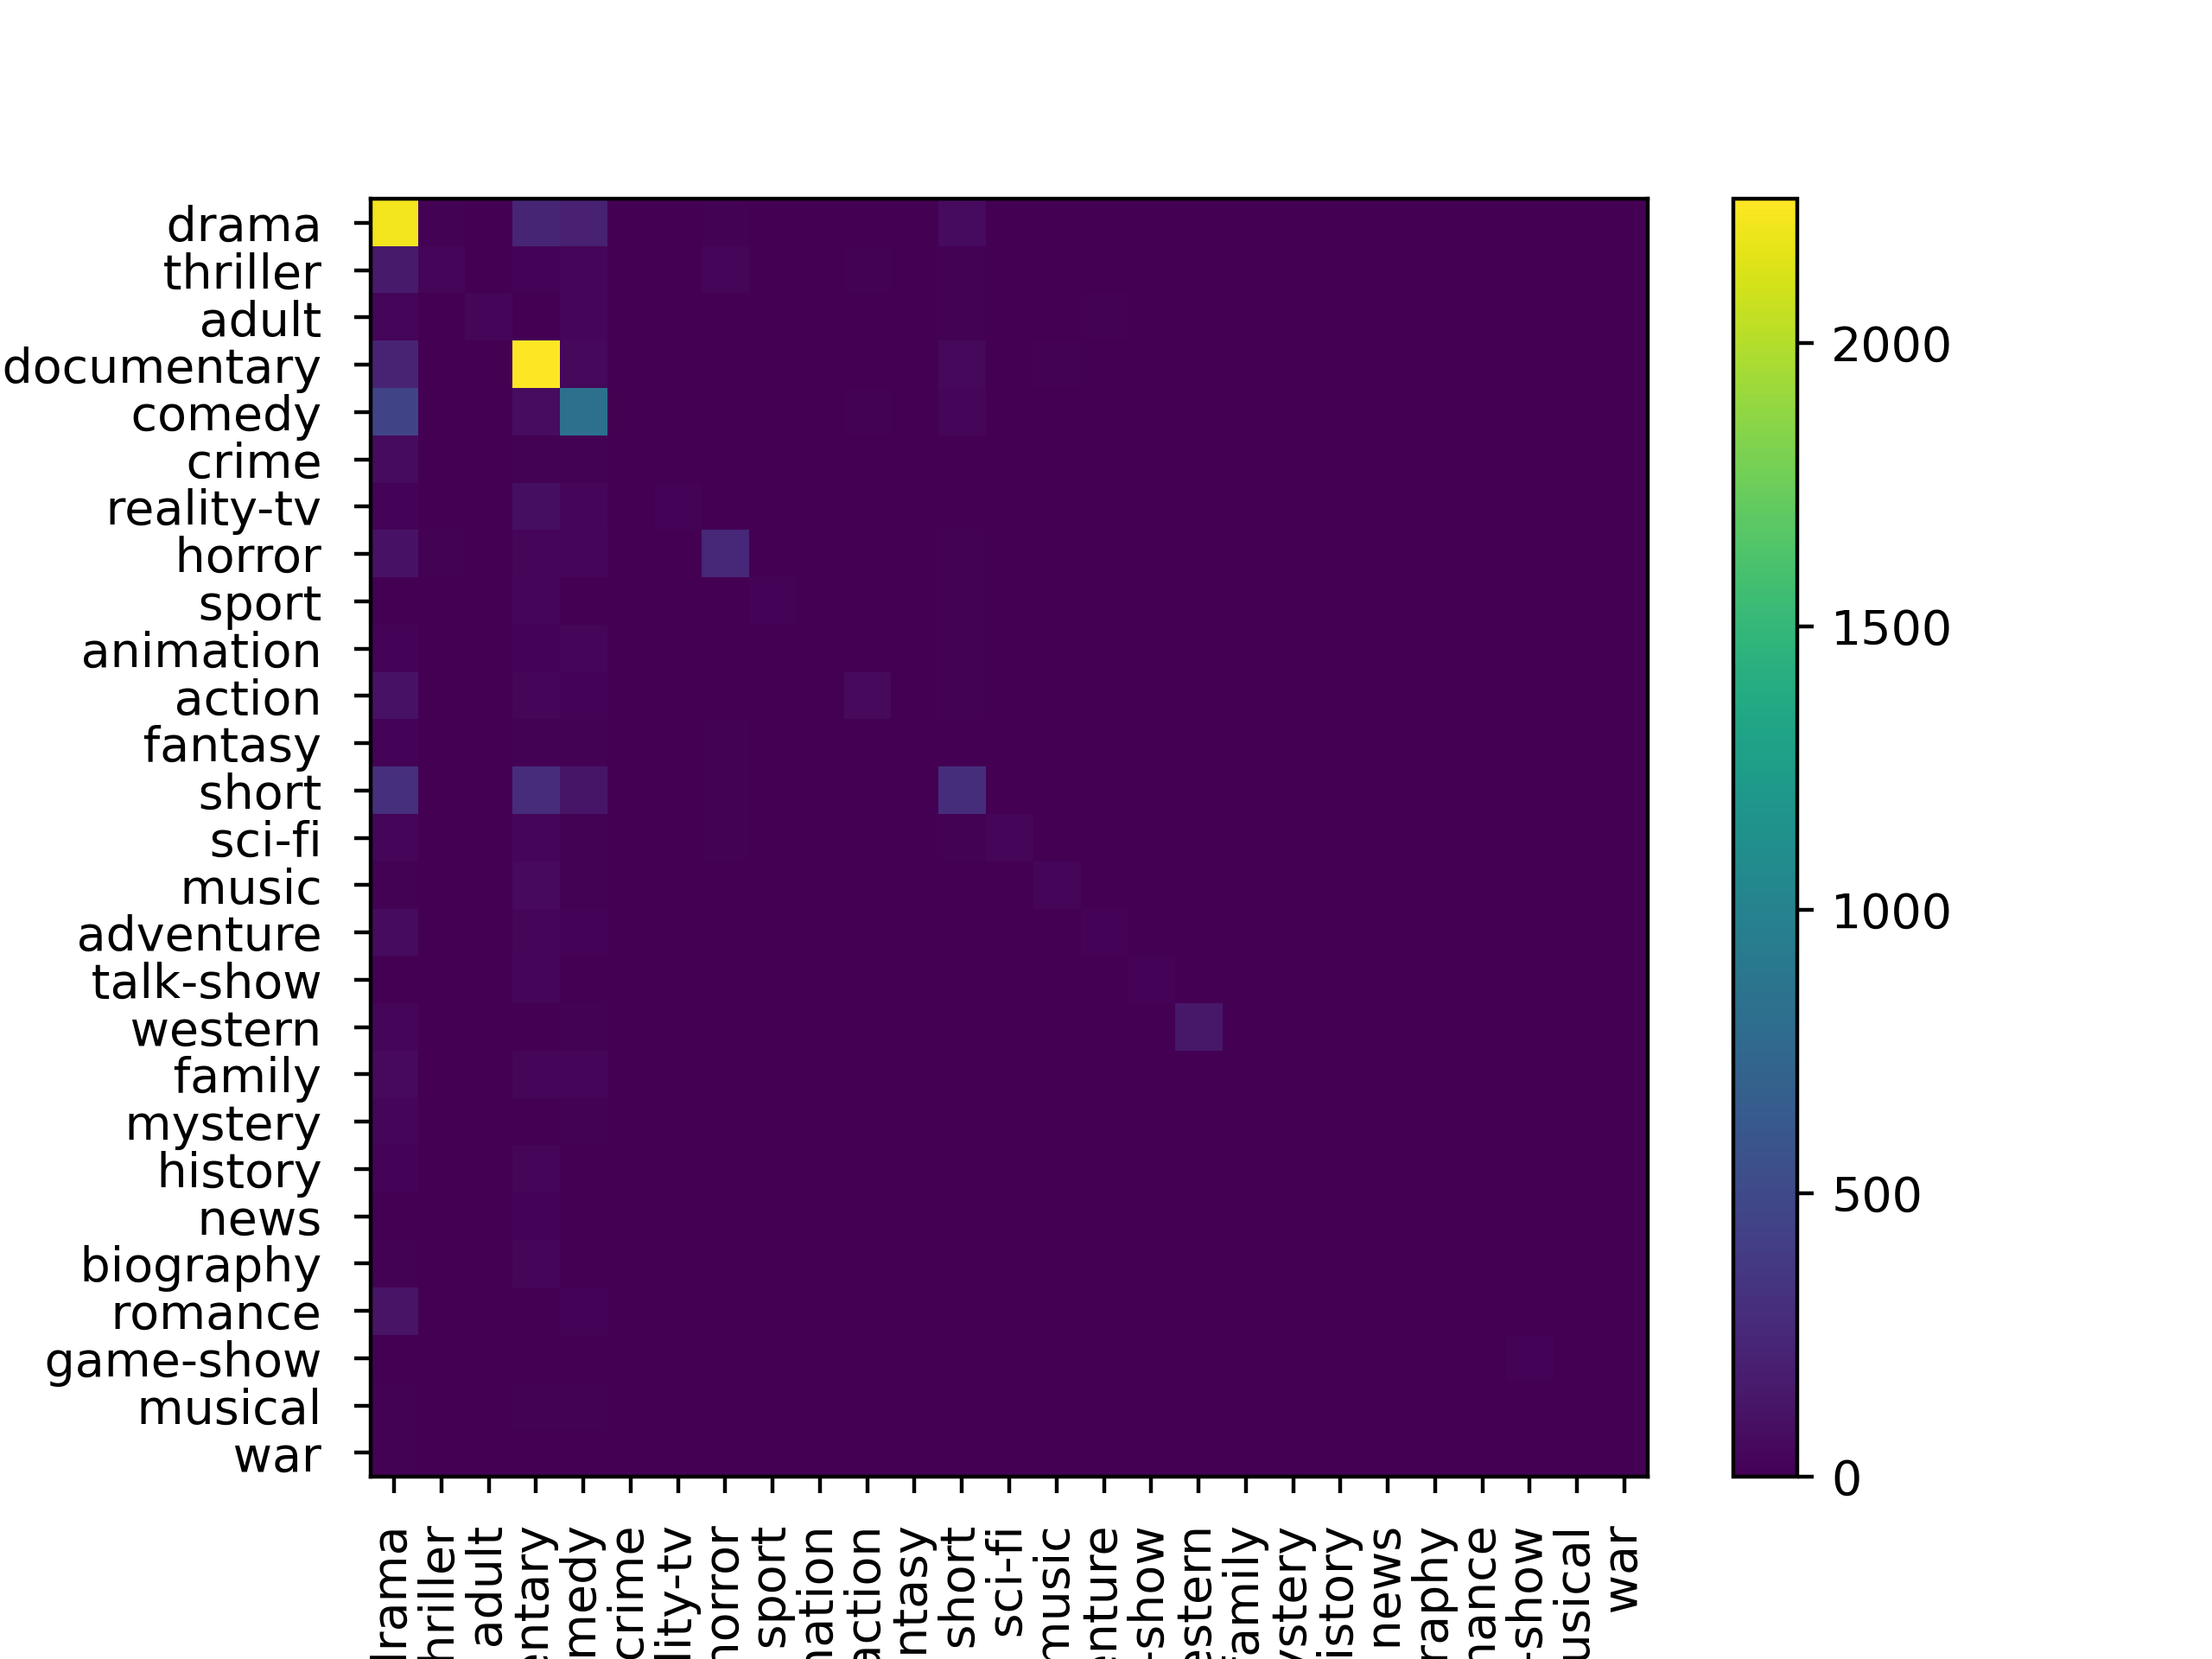
\includegraphics[scale=1]{graphs/confusion_matrix_LogisticRegression().png}
    \captionof{figure}{Matrice de Confusion LogisticRegression}
\end{center}
On peut voir que malgré le changement de classification la confusion concernant \textbf{Drama} et \textbf{Documentary} persiste. 
















\newpage
\subsection{MLPClassifier}

Multi-layer Perceptron Classifier étant un modèle de réseau de neurones nous avons choisi de l'utiliser car l'objectif premier lorsque nous avons commencé le projet était d'en utiliser un pour prédire le genre.

\begin{center}
    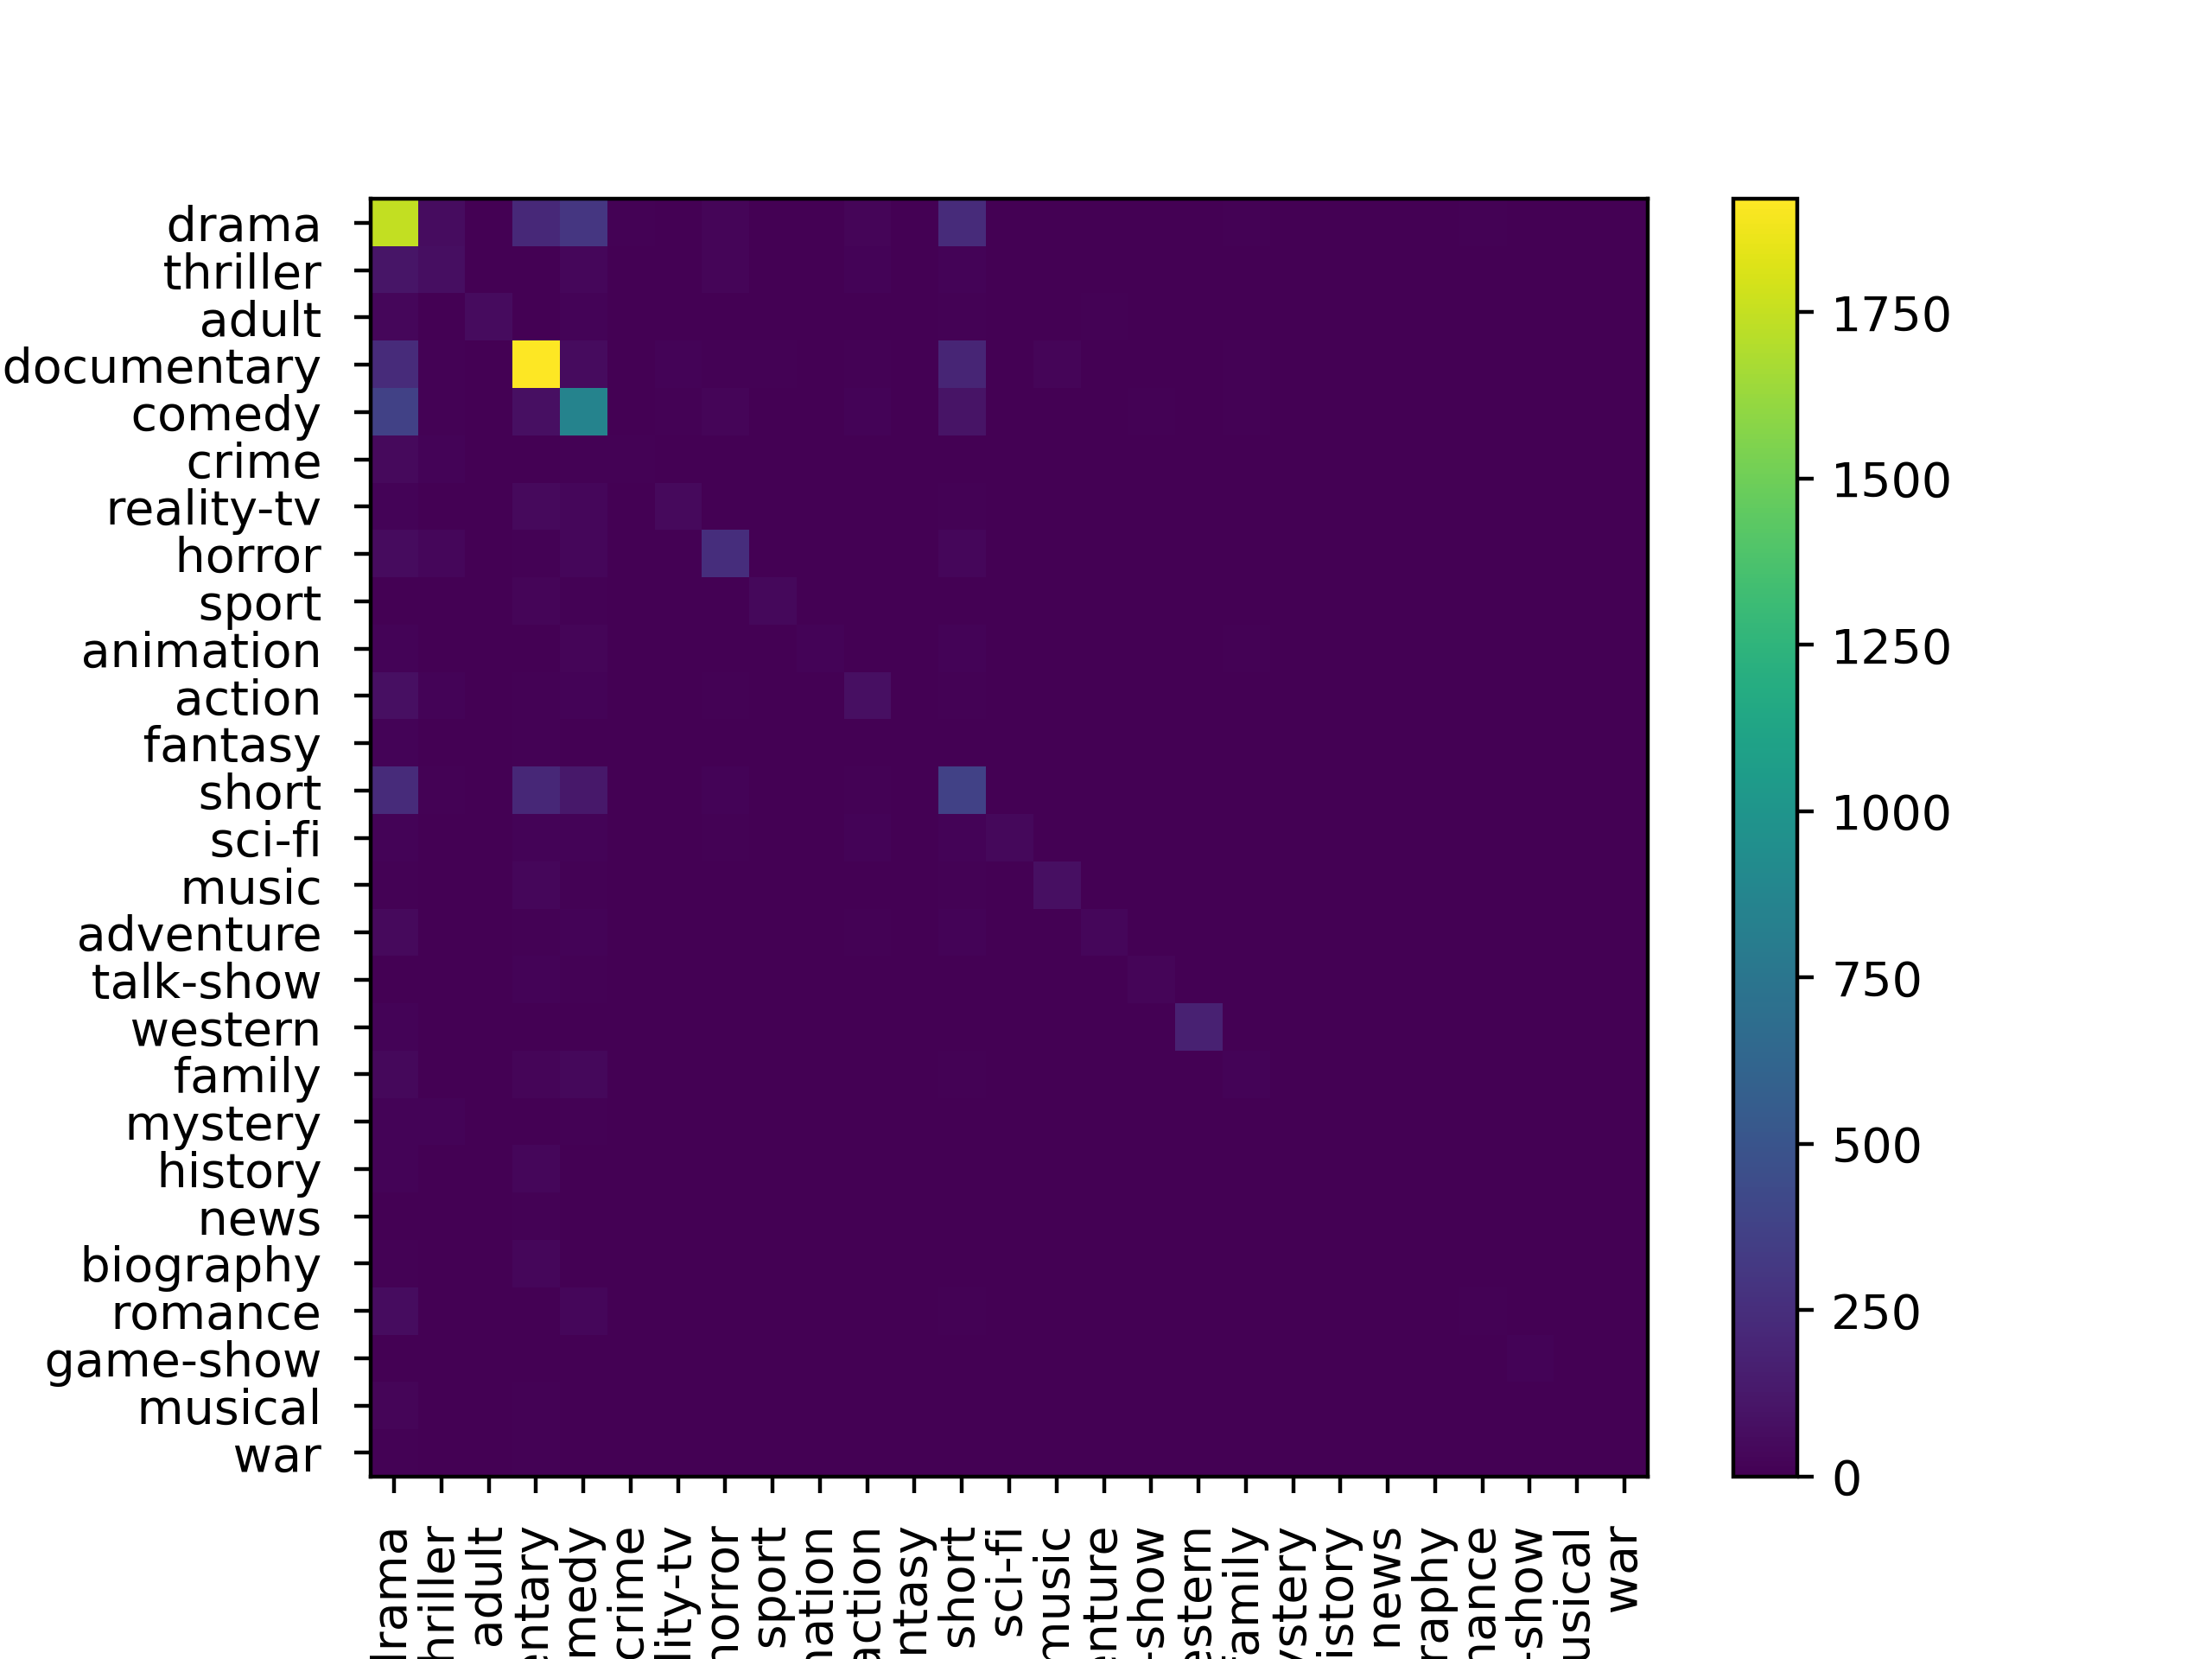
\includegraphics[scale=1]{graphs/confusion_matrix_MLPClassifier(hidden_layer_sizes=(46,)).png}
    \captionof{figure}{Matrice de Confusion MLPClassifier}
\end{center}

Là aussi pour la matrice de confusion le problème est le même qu'auparavant, nous pouvons tout de même dénoter une accentuation sur le genre \textbf{comedy} et une baisse sur \textbf{drama}.